\chapter{Multivariate and Large Benchmark Datasets}
\label{apd:multivariate_datasets}

In recent years the search for renewable energy sources has grown and, as most of them are not perennial power sources, its integration on smart environments will require ability to predict their output generation.

In order to contribute with the research reproducibility, all data and source codes are available in the following URL \url{http://bit.ly/scalable_probabilistic_fts_appB}.


\section{SONDA dataset}

The Project SONDA - Sistema de Organização Nacional de Dados Ambientais (Brazilian National System of Environmental Data Organization), is a governmental project which groups environmental data (solar radiance, wind speed, precipitation, etc) from INPE - Instituto Nacional de Pesquisas Espaciais (Brazilian Institute of Space Research). The chosen variables are the global solar horizontal radiation and the wind speed at 10 meters, both from the Brasilia telemetry station\footnote{Code: BRB. Coordinates: 15\textdegree 36' 03" S 47\textdegree 42'47" O. Alt.: 1023m}, recorded between 2012 and 2015, by minute, summing 2 million instances. This dataset was retrieved directly from the SONDA Project page at \url{http://sonda.ccst.inpe.br/}\footnote{Access in 19/05/2019}

\begin{table}[htb]
    \centering
    \begin{tabular}{|c|c|l|} \hline
        \textbf{Variable} & \textbf{Type} & \textbf{Description}  \\ \hline
        DateTime & Time Stamp & yyyy-MM-dd HH:MM  \\ \hline
        glo\_avg & Real & Global average solar radiation in   \\ \hline
        ws\_10m & Real & Wind speed in meters by second (m/s)  \\ \hline
    \end{tabular}
    \caption{SONDA dataset variables}
    \label{tab:sonda_variables}
\end{table}

\begin{figure}[htb]
    \centering
    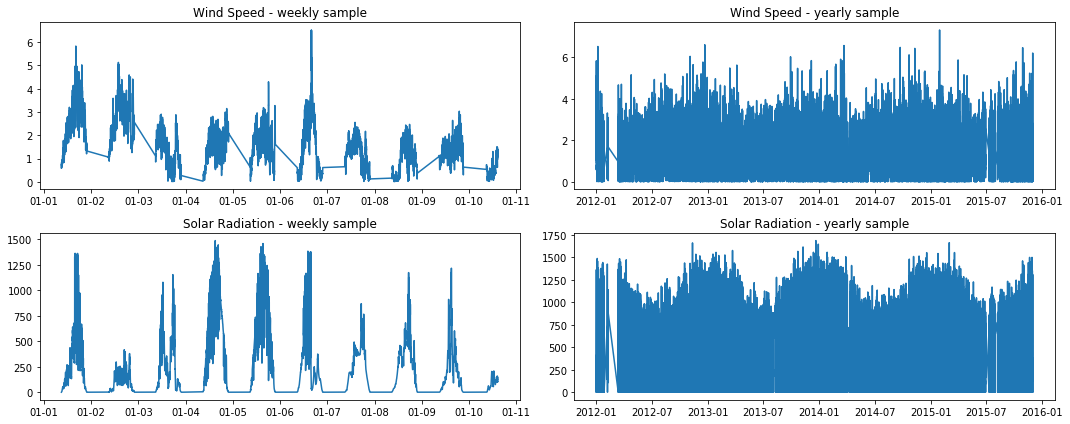
\includegraphics[width=\textwidth]{figures/dataset_sonda.png}
    \caption{SONDA dataset samples}
    \label{fig:sonda}
\end{figure}

\begin{figure}[htb]
    \centering
    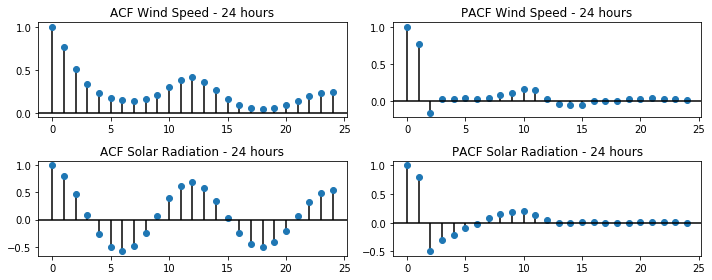
\includegraphics[width=\textwidth]{figures/dataset_sonda_acf.png}
    \caption{Autocorrelation and Partial Autocorrelation plots for SONDA dataset}
    \label{fig:sonda_acf}
\end{figure}

\section{Malaysia dataset}

Hourly electric load and temperature data of the power supply company of the city of Johor in Malaysia sampled between 2009 and 2010, with 17,519 instances. This dataset was retrieved from \cite{Sadaei2019}.

\begin{table}[htb]
    \centering
    \begin{tabular}{|c|c|l|} \hline
        \textbf{Variable} & \textbf{Type} & \textbf{Description}  \\ \hline
        DateTime & Time Stamp & yyyy-MM-dd HH:MM  \\ \hline
        temperature & Real & Temperature in Celcius degrees ($^o$C) \\ \hline
        load & Integer & Eletric load in Mega Watts by hour (MW/h)  \\ \hline
    \end{tabular}
    \caption{Malaysia dataset variables}
    \label{tab:malaysia_variables}
\end{table}

\begin{figure}[htb]
    \centering
    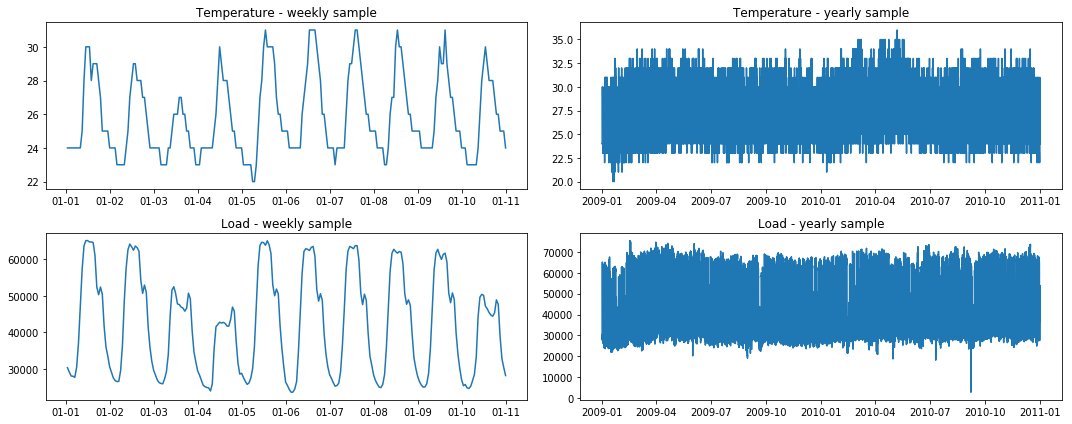
\includegraphics[width=\textwidth]{figures/dataset_malaysia.png}
    \caption{Malaysia dataset samples}
    \label{fig:malaysia}
\end{figure}

\begin{figure}[htb]
    \centering
    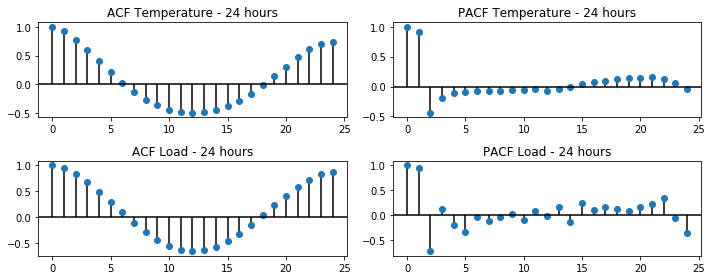
\includegraphics[width=\textwidth]{figures/dataset_malaysia_acf.png}
    \caption{Autocorrelation and Partial Autocorrelation plots for Malaysia dataset}
    \label{fig:malaysia_acf}
\end{figure}

